\documentclass{article}

% You can use any LaTeX packages here
\usepackage{graphicx}
\usepackage{hyperref}
\usepackage[top=0in, right=0.4in, left=0.4in, bottom=0.4in]{geometry}
\usepackage{tikz}
\usepackage{multicol}
\usepackage{lettrine}

\usepackage[T1]{fontenc}
\usepackage{fourier}


% some random thing to fix Rmd issues
%
\renewcommand{\topfraction}{.85}
\renewcommand{\bottomfraction}{.7}
\renewcommand{\textfraction}{.15}
\renewcommand{\floatpagefraction}{.66}
\setcounter{topnumber}{3}
\setcounter{bottomnumber}{3}
\setcounter{totalnumber}{4}

\setlength{\parskip}{0pt} % eliminate spacing between paragraphs

\begin{document}

\pagenumbering{empty}
\pagestyle{empty}

\definecolor{msugreen}{HTML}{008208}


\newcommand{\mycbox}[1]{\tikz{\path[draw=msugreen,fill=msugreen] (-1,0) rectangle (8cm,0.7cm);}}

\newcommand{\econbox}[1]{\tikz{\path[draw=msugreen,fill=msugreen] (0,0) rectangle (0.2cm,0.2cm);}}

\newcommand{\helmet}{
\includegraphics[height=1.1em]{spartan.jpg}}

\mycbox  \par\noindent\hspace*{0.5cm}\rule{0.489\textwidth}{0.5pt}

%\hspace{4em}

\begin{minipage}[c]{0.5\textwidth}
    \begin{flushleft}
    \makeatletter
    {\fontfamily{phv}\selectfont{\Large \textcolor{msugreen}{Graphic Detail}: Inequality}}
    \makeatother
    \end{flushleft}
    \end{minipage}
    \begin{minipage}[t]{0.4\textwidth}
    \begin{flushright}
    \makeatletter
    {\fontfamily{phv}\selectfont{\textbf{Andy Halterman} September 13
2024}}
    \makeatother
    \end{flushright}
    \end{minipage}
    
    \begin{center}
    \par\noindent\rule{\textwidth}{0.5pt}
    \end{center}
        
    \begin{center}
    \includegraphics[width=\textwidth]{placeholder\_figure.jpeg}
    \end{center}

    \begin{multicols}{3}
    \makeatletter
    \noindent {\Large \textbf{Inequality and standard of living}}
    \makeatother 
    \vspace{0.2in}
    
    \noindent {\textbf{If US inequality were like Germany's, everyone
would have a good standard of living.}}
    
    \vspace{0.15in}
    
    \emph{Tip from last year's students}: As soon as you get this file,
knit it as-is. That will give you plenty of time to debug any
compilation/LaTeX issues.

You'll have a separate Rmd file where you'll do your analysis and create
your figures. Then you'll save out the figure to a file and include it
here, along with your writeup.

You'll replace this text with your own text. You can use Markdown to
format your text. Some things to note about this template:

You'll need to ensure that \texttt{econ\_template.tex} \emph{and}
\texttt{spartan.jpg} are both in the same folder as this file.

Above, in the block of code inside the \texttt{-\/-\/-} marks, you'll
see \texttt{placeholder\_figure.jpeg}. You'll replace that with the name
of your own figure file that you produce. Make sure that the file ending
matches: you'll probably have a \texttt{.png} or \texttt{.pdf} file. So
if I ran my analysis code to generate a figure called
\texttt{figure\_397\_ccc.png}, I'd replace
\texttt{figure\_path:\ placeholder\_figure.jpeg} with
\texttt{figure\_path:\ figure\_397\_ccc.png}. Your main figure should
include 2-3 figures, compiled neatly into a single figure using
patchwork. You'll need to experiment to get the layout and size right.
You might need to go through a few steps of saving the combined
patchwork plot out (using \texttt{ggsave()}) and opening up the image to
make sure it looks right.

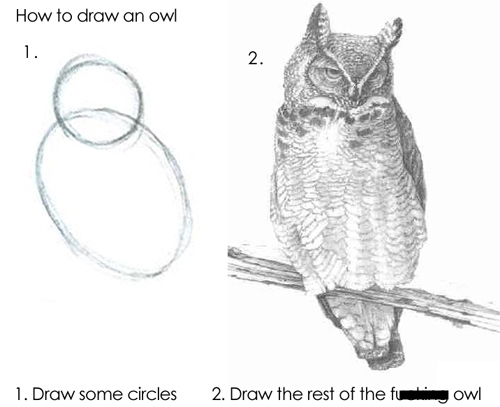
\includegraphics[width=0.95\columnwidth]{owl.jpg}

Make sure you change the ``title'' and ``tag'' fields to match your
content. It's okay to have some fun with the title! The ``summary'' text
goes in bold at the beginning of your document and should do what it
says: summarize the main takeaway of your piece in a sentence.

If you want to include an extra, small figure inside the text (very
optional!!), you can do that, too. Replace \texttt{owl.jpg} with your
second small figure. You'll need to experiment with where you place the
\texttt{\textbackslash{}includegraphics} command to get the placement
right. If you don't want to include another figure, just delete the
\texttt{\textbackslash{}includegraphics} line.

Here's some filler text from CCC's Github to round out the page:

``We strive to update this data set weekly, on Wednesdays not later than
4 PM Eastern time, with exceptions around holidays and ends of months.
Please note that, while the raw data are updated on a rolling basis,
there is some lag between the appearance of a news story or social-media
post about an event (or the submission of a form to CCC) and the
addition of a complete record to CCC's Google Sheets. CCC strives to
keep that interval as short as possible, but the project operates on a
shoestring budget, so periods of higher protest activity can make for
longer delays.''~\helmet %\econbox{red}
    \end{multicols}

    
\end{document}
